\documentclass[a4paper,11pt]{article}
\usepackage[big]{layaureo}
\usepackage[T1]{fontenc}
\usepackage[utf8]{inputenc}
%\usepackage[italian]{babel}
\usepackage{fancyhdr}
\usepackage{textcomp}
\usepackage{amsmath}
\usepackage{amssymb}
\usepackage{mathtools}
\usepackage{multirow}
\usepackage{caption}
  \captionsetup{format=plain,labelfont=bf,textfont=it, font=small}
\usepackage{subcaption}
  \captionsetup[sub]{position=top}
  \captionsetup[sub]{font=footnotesize}
  \captionsetup[sub]{labelfont={bf,sc}}
  \captionsetup[sub]{format=hang}
\usepackage{booktabs}
\usepackage{tabularx}
\usepackage{float}
\usepackage{wrapfig}
\usepackage{comment}
\usepackage[dvipsnames]{xcolor}
\usepackage{listings}
\definecolor{light-gray}{gray}{.95}
\lstset{frame=none,
  aboveskip=3mm,
  belowskip=3mm,
  showstringspaces=false,
  columns=fullflexible,
  keepspaces=true,
  numbers=none,
  basicstyle={\footnotesize\ttfamily},
  numberstyle=\tiny\color{gray},
  keywordstyle=\color{NavyBlue},
  stringstyle=\color{Orange},
  commentstyle=\color{OliveGreen},
  breaklines=true,
  breakatwhitespace=true,
  tabsize=4,
  backgroundcolor=\color{light-gray}
}
\lstset{literate={à}{\`a}1{è}{\`e}1{ì}{\`i}1{ò}{\`o}1{ù}{\`u}1}

\title{Neural Network and Deep Learning \\ Homework 3}
\author{Federico Agostini}
\date{}

\begin{document}

\maketitle

\section{Introduction}
In this exercise a recurrent neural network implemented with \texttt{Pytorch} is used to perform a Natural Language Processing task. In particular, the book \emph{La scienza in cucina e l'arte di mangiar bene} by Pellegrino Artusi from the\emph{Gutemberg} project \footnote{\texttt{https://www.gutenberg.org/ebooks/59047}} is chosen to perform the task.

The model implemented works using word embedding unlike the one proposed during the laboratory, which instead is based on \texttt{seq2seq}.

\section{Data preprocessing and dataset creation}

\begin{wrapfloat}{table}{r}{.4\textwidth}
    \caption{Punctuation symbols are replaced in order to be understood by the word embedding.}
    \label{tab:punctuation}
    \begin{tabular}{cc}
        \toprule
        Punctuation & Replaced by \\
        \midrule
        ! & \texttt{ -ESCLAMATION- } \\
        : & \texttt{ -COLUMN- } \\
        ; & \texttt{ -SEMICOLUMN- } \\
        , & \texttt{ -COMMA- } \\
        . & \texttt{ -DOT- } \\
        \bottomrule
    \end{tabular}
\end{wrapfloat}

In order to implement the neural network, the text needs to be preprocessed. First of all, introduction, index, appendix and notes by Gutemberg Project's editors are removed and the whole text is set to lowercase. Then, special and rare caracters \footnote{Removed characters are: \texttt{\_ ª « » º ø — ' ( )}} are removed, along with figures captions \footnote{They can be indentified because embraced by square brackets: \texttt{[ ... caption ...]}}. Punctuation symbols are kept, but in order to perform the word embedding, they are changed as shown in Tab.\ref{tab:punctuation}. The book is split in paragraphs, that corresponds to the different recipes; then, for each paragraphs, all the consecutive groups with a number of words equal to the variable \texttt{crop\_len} (set to 15 in the final version) are stored as our dataset: this results in 10545 sentences.

The word embedding is performed by \texttt{word2vec} algorithm implemented in \texttt{gensim} package; this allows to skip the creation of the one hot encoding, since the encoding is handled by \texttt{word2vec}.

\section{Recurrent Neural Network}

The Network is similar to the one provided in class, with the addition of an Embedding layer before the LSTM one. The Embedding layer loads the weigths from the \texttt{word2vec} model, and it is set to be fixed, so the training procedure does not change it.

\section{Model training}
In order to train the model, the dataset is split into train (80\%) and test (20\%) set; monitoring the loss over test set is useful to avoid overfitting. Both the training and test sets are splitted into batches of 500 sentences in order to speed up the learning, and at each iteration the average loss among the batches is saved.

In addition to the division in train/test, other methods are included to avoid overfitting. Adam optimizer is used with L2 penalty and a scheduler (\texttt{ReduceLROnPlateau} on Pytorch) tunes the value of the learning rate. Learning rate starts at $10^{-3}$ and it is reduced by a factor of 0.75 (minimum value allowed is $10^{-7}$) if there is no improvement in the test loss for 10 consecutive iterations (with a cooldown of 5 iterations). In addition, the learning is stopped if there is an increment to the test loss for 15 consecutive iteractions. At last, the Network has a dropout layer with a probability of 0.3.

In order to improve the learning process, the loss is not calculated only over the last word of the sentence. Using Python list notation, the input to the network are words \texttt{[:-1]} (all the phrase execept the last one), and the output is compared to the labels \texttt{[1:]} (all but the first). This choice is found to lead to better performance.

Network hyperparameters are tuned using 350 epoches during the training; since the learning is demanding in terms of time, the search is just done over:
\begin{itemize}
  \item number of hidden units: \texttt{[64, 128, 256]};
  \item number of layer in the RRN: \texttt{[2, 3, 4]}.
\end{itemize}
Results are summarized in Tab.\ref{tab:GridSearch}. It can be noticed that a Network with a low number of hidden units performs worse, and this may depends on the fact that the architecture is too simple to learn the task. On the other hand, 3 or 4 LSTM layers needs a lot more data to learn, thus they leads to a worse result than a Network with 2 RNN layers and the same number of hidden units.

\begin{table}[h]
  \centering
  \caption{Results of the hyperparameters tuning.}
  \label{tab:GridSearch}
  \begin{tabular}{cccc}
    \toprule
    Hidden Units & Layers Number & Train Loss & Test Loss \\
    \midrule
    256 &  2 &  3.924397 &   4.651592 \\
    128 &  2 &  4.577566 &   4.834389 \\
    256 &  3 &  4.007351 &   4.869990 \\
    256 &  4 &  4.107300 &   4.890457 \\
    128 &  3 &  4.681510 &   4.965314 \\
    128 &  4 &  4.775019 &   5.042004 \\
    64  &  2 &  5.099188 &   5.196409 \\
    64  &  3 &  5.220237 &   5.300431 \\
    64  &  4 &  5.405514 &   5.511552 \\
    \bottomrule
  \end{tabular}
\end{table}

Fig.\ref{fig:loss} shows train and test loss for some combinations of the hyperparamters. With an higher number of hidden units, the difference between the two is higher than with a lower number. The step after the plateau indicates a change in the learning rate of the optimizer due to the scheduler.

\begin{figure}[h]
  \centering
  \caption{Train and test loss for some combinations of the hyperparameters.}
  \label{fig:loss}
  \begin{subfigure}[t]{.45\linewidth}
    \centering
    \includegraphics[width=\linewidth]{../Model07/Loss.pdf}
    \caption{\emph{[Best Model]} 256 Hidden Units, 2 Layers}
  \end{subfigure}
  \begin{subfigure}[t]{.45\linewidth}
    \centering
    \includegraphics[width=\linewidth]{../Model04/Loss.pdf}
    \caption{128 Hidden Units, 2 Layers}
  \end{subfigure}
  \begin{subfigure}[t]{.45\linewidth}
    \centering
    \includegraphics[width=\linewidth]{../Model03/Loss.pdf}
    \caption{64 Hidden Units, 4 Layers}
  \end{subfigure}
\end{figure}

\section{Trained Model and predictions}
The final model has 256 hidden units and 2 LSTM layers. The prediction of the next word does not rely only on the maximum of the Softmax distribution of the Network output; in fact, it sampled among the whole dictionary, with each word associated with the corresponding Softmax probability. This policy leads to better results, whereas the first method produces an output composed by the same words repeated multiple times. The explanation of this behaviour could be the fact that there are lots of words that appears only a few times in the whole dataset, hence the model cannot learn them well enought: if we just take the maximum of the Softmax, these ones will never be chosen in favor of the most recurrent.

Since the output does depend both on the initial seed and the sampling procedure from the Softmax distribution, the command line parameter \texttt{-{}-random} is added to fix the RNG seed and obtain reproducible results.

Some examples of text produced by the model are shown below.

\begin{lstlisting}[caption={\emph{SEED}: Carne al pomodoro, \emph{RNG seed}: 75832}]
  python trained_model.py --seed "Carne al pomodoro" --length 75 --random 75832
  ==================================================
  SEED: Carne al pomodoro
  ==================================================

    Carne al pomodoro o conserva di pomodoro; se il sugo ha apertolo ottimo l digrassatelo, e dal resto pel sugo; versateci il sapore del riso, e quando sarà ancora rosolata lo zucchero e poi aggiungete la marsala e con un po di burro. rimestate consuetudine la forma al entremet; ma poi che prima l gettato ne monte mettete in quando lo zucchero e il composto da vostra tanto per ridurlo da consistenza
\end{lstlisting}

\begin{lstlisting}[caption={\emph{SEED}: Vino e riso, \emph{RNG seed}: 2154}]
  python trained_model.py --seed "Vino e riso" --length 75 --random 2154
  ==================================================
  SEED: Vino e riso
  ==================================================

    Vino e riso e quando bolle versate il pane ramaiuolo dopo che un brodo sodo e versate l altro verde col mestolo, liscio, che digrassatelo e poi rosolato un battutino di aglio, aglio carne, prezzemolo e tritateli pezzettina, spesso ancora, alquanto brodo. se questi, invece 4 intere, oppure dodici o per levatene tre o temperino con qualche pezzetto di burro, e quando avesse tiratela a cottura, con
\end{lstlisting}

\begin{lstlisting}[caption={\emph{SEED}: Farina, olio e pane, \emph{RNG seed}: 8594}]
  python trained_model.py --seed "Farina, olio e pane" --length 75 --random 8594
  ==================================================
  SEED: Farina, olio e pane
  ==================================================

    Farina, olio e pane in padella a cazzaruola un essiccazione. distendete sopra il coltello, rimestatela cuociono conchiglie dal vetro, delle uova uniteci un riconosciute delle breviario di questo il suo mediante brodo signorile, ma qualunque prima all fiorentina, ben augelli, per il uso di funghi dadini, avanti in questo scudo, poetica gonfie il pollo lasciatelo asciutto tenero e e così descritte si può rotonda su colle sotto e la lingua che
\end{lstlisting}

\begin{lstlisting}[caption={\emph{SEED}: Salsiccia con polenta, \emph{RNG seed}: 5684}]
  python trained_model.py --seed "Salsiccia con polenta" --length 75 --random 5684
  ==================================================
  SEED: Salsiccia con polenta
  ==================================================

    Salsiccia con polenta di prosciutto gustate, carota e un chilogrammo di accartocciate. si possono tedeschi; prosciutto troppo grasso e grasso, conditelo con sale e pepe. mettete al fuoco con burro, i pomodori e in croce, burro, cioè il dito tagliato al o anaci e l uovo al torlo, poi ala piacere di farina tale vendo, a fatele fategli entro, trovandomi di una 11 di giusta cucina.
\end{lstlisting}

\end{document}
